\chapter{Proposta}\label{chp:PROPOSTA}

% falar sobre o capitulo

\section{Motivação}

% Intro
% SINAES

No Brasil, desde 2004 por meio da Lei n° 10.861 as instituições de ensino superior devem estar de acordo com as normas do Sistema Nacional de Avaliação da Educação Superior (SINAES)
cujo objetivo é contribuir para a melhoria contínua dos cursos e instituições avaliando 
os aspectos relacionados ao ensino, pesquisa, extensão, do corpo docente, da gestão institucional, bem como a responsabilidade social e infraestrutura.

% Problema: SINAES mt abrangente

A avaliação institucional desempenha um papel crucial na melhoria contínua da qualidade educacional
e é uma tarefa complexa que demanda a consideração de vários fatores. Embora o SINAES seja fundamental para esse processo no Brasil, sua metodologia geral de avaliação é aplicada a todas as áreas do conhecimento, o que pode não levar em conta especificidades de determinadas áreas.

% Problema: 

Os discentes são os principais protagonistas desse processo, sendo diretamente impactados pelas disciplinas cursadas e pelos professores que as ministraram. Ao avaliar esses elementos, os estudantes podem manifestar suas opiniões, pontuar se o conteúdo está alinhado às expectativas e se é relevante para sua formação. Além disso, uma avaliação do professor possibilita uma análise aprofundada do seu desempenho, levando em conta didática, comunicação e capacidade de estimular o interesse do aluno.

% Mas pq um sistema web? %
% -> Privacidade do aluno ao dar o feedback
% -> Agilidade e eficiencia na coleta e análise dos dados
% -> Acompanhamento em tempo real 
% -> Fácil acesso

% Solução: Sistema próprio da universidade de avaliação

Não restam dúvidas quanto à relevância das universidades no progresso do país, sendo necessário uma administração adequada e alinhada às exigências. Nesse sentido, as universidades devem se esforçar para estabelecer um sistema interno de garantia da qualidade que, na verdade, forneça uma base genuína para a tomada de decisões gerenciais. \citeonline{selfEvaluation2012}

Para que a instituição esteja preparada para enfrentar desafios, é fundamental que seus membros tenham ciência de sua realidade, virtudes, capacidades e limitações.
%Nelson de Abreu Júnio[2] (2009)
Segundo \citeonline{nelsonAbreu2009}, os processos avaliativos precisam envolver o maior número de participantes, tanto na construção de seu projeto quanto na análise e no uso dos resultados, contribuindo para o desenvolvimento humano.

A melhoria dos sistemas de ensino superior em países em desenvolvimento requer uma autoavaliação. Nesse contexto, e de acordo com \citeonline{betts1992}, há a necessidade de desenvolver uma capacidade aumentada de autoreflexão, autodireção e autorrenovação no ambiente de ensino superior. Tornando-se fundamental que a avaliação institucional seja realizada de forma automatizada pelas próprias instituições de ensino.

A utilização de sistemas e plataformas digitais permite que as universidades coletem, processem e analisem os dados de maneira precisa e eficiente, espeitando a privacidade dos alunos. Além disso, a automação desse processo reduz o tempo necessário para a obtenção dos resultados, permitindo que a instituição colete os dados quantitativos e qualitativos de maneira abrangente, envolvendo um maior número de estudantes.

%\cite{braida2015transforming}
%\citeonline{braida2015transforming}

% justificar melhor o trabalho

\section{Trabalhos Relacionados}
Neste tópico serão apresentados alguns sistemas de avaliação aplicados por universidades e trabalhos acerca da avaliação institucional no ensino superior.

De uma maneira mais geral, temos o \textit{Rate my Professors}\footnote{\url{https://www.ratemyprofessors.com/}}, que foi criado
com a motivação de ajudar outros estudantes universitários a tomar decisões informadas ao escolher suas aulas e professores, acreditando que as opiniões dos alunos poderiam ajudar futuros alunos, tornando a seleção de aulas e professores mais transparente e informada.

A Universidade Federal Fluminense (UFF) possui a Comissão Própria de Avaliação Institucional da UFF (CPA/UFF),
responsável pela formulação do instrumento de avaliação da Universidade, conhecido como Sistema de Avaliação Institucional (SAI).
O SAI foi desenvolvido com o propósito de coletar a perspectiva dos alunos e professores sobre os cursos de graduação,
mediante a avaliação do desempenho efetivo nas disciplinas e da disponibilidade de infraestrutura para o seu funcionamento.
Os resultados obtidos por meio dessa avaliação são analisados pela CPA/UFF, pelas Unidades Acadêmicas, pelos Departamentos de Ensino e pelas Coordenações de Curso,
e servem como base para a reflexão acerca da qualidade do trabalho acadêmico realizado na UFF, gerando informações relevantes e necessárias para a reformulação dos Projetos Pedagógicos dos Cursos.



% Falar sobre universidades que aplicam avaliações internas:
% Exemplo: 
% Universidad de Buenos Aires (UBA)
% Universidade de São Paulo (USP) = Avaliação Institucional da USP
% Universidade Federal FLuminense (UFF) = Avaliação Institucional da UFF


\section{Proposta}

Esse capítulo propõe um sistema web de avaliação de disciplinas para o curso de Ciência da Computação da UFRRJ, com o objetivo de auxiliar o departamento do curso a tomar decisões que visem melhorar o ensino e aprendizado dos alunos.

O intuito desse trabalho é desenvolver um sistema web onde os alunos da Universidade Federal Rural do Rio de Janeiro possam avaliar as disciplinas ofertadas ao longo do período. O sistema permite que os aluno acessem um questionário de avaliação para cada disciplina em que ele estava matriculado. Esse questionário conta com perguntas que podem medir a qualidade da didática do professor, a ementa da disciplina, as avaliações, entre outros.

O sistema conta com uma tela de cadastro que pode ser usada tanto por alunos e professores da universidade e uma tela de login. Caso o usuário logado seja um aluno, ele poderá visualizar uma lista das disciplinas em que ele estava matriculado. O aluno pode avaliar cada disciplina dessa lista somente uma vez. Caso o usuário logado seja um professor, ele terá acesso a uma lista de disciplinas lecionadas por ele. Cada disciplina contará com um relatório com a média de avaliações recebidas. Caso o usuário seja um administrador, ele poderá acessar todas as disciplinas do curso de Ciência da Computação da UFRRJ, e visualizar o relatório de avaliações para cada uma delas.

Administradores do sistema poderão cadastrar períodos e disciplinas, e associar os professores a suas respectivas disciplinas. 

\subsection{Atores}
Um ator é uma entidade externa que interage com o sistema e desempenha um papel específico dentro do contexto do sistema em análise.

Ao identificar os atores, é possível determinar quais são as suas responsabilidades e como eles se relacionam com as funcionalidades do sistema. Essas informações são utilizadas para modelar os casos de uso e requisitos do sistema.

Com base na proposta apresentada anteriormente, é possível identificar os seguintes atores:

\begin{alineas}
  \item Aluno: Representa os alunos do curso de Ciência da Computação. Eles podem visualizar a lista de disciplinas em que estão matriculados e avaliá-las uma vez.
  \item Professor: Representa os professores responsáveis pelas disciplinas do curso. Eles podem visualizar as disciplinas que lecionam e um relatório com as avaliações recebidas para cada uma delas.
  \item Coordenador: Representa o(s) coordenador(es) do curso. Eles têm a responsabilidade de cadastrar disciplinas, associar os professores às disciplinas ministradas por eles, e, principalmente, visualizar relatórios com as avaliações de cada disciplina. Esses relatórios são fundamentais para análise de resultados e tomadas de decisões estratégicas para melhorar a qualidade do curso.
\end{alineas}

Esses atores desempenham papéis distintos no sistema de avaliação de disciplinas, e cada um contribui de uma maneira para o funcionamento do sistema.

\subsection{Regras de Negócio}
As regras de negócio definem diretrizes e restrições de uma aplicação. Elas são essenciais para que haja clareza do que deve ser feito ao desenvolver um sistema, atendendo às necessidades e requisitos do negócio.

Algumas das regras de negócio aplicadas ao sistema de avaliação de disciplinas são:

\begin{alineas}
  \item \textbf{RN1 - Restrição de matrícula} O Aluno só pode avaliar em que ele esteja matriculado: Não é permitido avaliar disciplinas não cursadas.
  \item \textbf{RN2 - Restrição de avaliação única} O Aluno só pode avaliar uma disciplina uma única vez: Cada disciplina pode ser avaliada somente uma vez por cada aluno.
  \item \textbf{RN3 - Restrição de anonimato} O Aluno não pode ser identificado na avaliação: A avaliação deverá ser anônima.
  \item \textbf{RN4 - Restrição de acesso aos relatórios} O Professor pode visualizar somente os relatórios de suas disciplinas: Não é permitido acessar relatórios de outros professores.
  \item \textbf{RN5 - Acesso do Coordenador aos relatórios} O Coordenador pode ver relatórios de todas as disciplinas: O Coordenador deve ter uma visão geral com todos os relatórios de avaliações das disciplinas do curso.
  \item \textbf{RN6 - Cadastro de disciplinas} O Coordenador pode cadastrar disciplinas: Somente o Coordenador pode realizar cadastros de disciplinas e associar professores a elas.
\end{alineas}

Esses exemplos destacam algumas das regras de negócio cruciais para o funcionamento do sistema de avaliação de disciplinas. Ao seguir essas regras, é possível desenvolver uma aplicação segura, eficiente e que respeite a privacidade dos dados dos usuários.

\subsection{Requisitos do Sistema}
Os requisitos do sistema são descrições sobre o que o sistema deve ser capaz de fazer para atender às regras de negócios. Esses requisitos são divididos em requisitos funcionais e não funcionais. 

Os requisitos funcionais especificam funcionalidades que o sistema deve ter para atender às necessidades do usuário final. Já os requisitos não funcionais especificam as restrições e limitações da aplicação.

Alguns requisitos funcionais do sistema de avaliação de disciplina são:

\begin{alineas}
    \item \textbf{RF1 - Cadastrar disciplina} O sistema permitirá que o Coordenador cadastre disciplinas informando NOME, TURNO, PROFESSOR e PERÍODO LETIVO.
    \item \textbf{RF2 - Editar disciplina} O sistema permitirá que o Coordenador edite o NOME, TURNO, PROFESSOR e PERÍODO LETIVO de uma disciplina.
    \item \textbf{RF3 - Excluir disciplina} O sistema permitirá que o Coordenador exclua uma disciplina.
    \item \textbf{RF4 - Listar disciplinas} O sistema permitirá a visualização de disciplinas (NOME, TURNO, PROFESSOR e PERÍODO LETIVO).
    \item \textbf{RF5 - Cadastrar período} O sistema permitirá que o Coordenador inclua um período letivo (ANO).
    \item \textbf{RF6 - Editar período} O sistema permitirá que o Coordenador edite o ano de um período letivo cadastrado no sistema.
    \item \textbf{RF7 - Excluir período} O sistema permitirá que o Coordenador exclua um período letivo.
    \item \textbf{RF8 - Visualizar relatórios} O sistema permitirá a visualização de relatórios de avaliações.
\end{alineas}

Ao satisfazer todos os requisitos do sistema, podemos garantir que o software é confiável e funcional. 

\begin{comment}
    \begin{table}[h]
        \centering
        \caption{Requisitos do Sistema}
        \label{tab:tabela_requisios_do_sistema}
        \resizebox{\textwidth}{!}{%
        \rowcolors{1}{}{lightlightgray}
        \begin{tabular}{ccc}
        \hline
        \textbf{ID} & \textbf{Nome} & \textbf{Descrição} \\ \hline
        \textbf{RF01} & Cadastrar disciplina & \begin{tabular}[c]{@{}c@{}}O sistema permiritá que o usuário inclua disciplina\\ informando NOME, TURNO, PROFESSOR, PERÍODO LETIVO\end{tabular} \\
        \textbf{RF02} & Editar disciplina & \begin{tabular}[c]{@{}c@{}}O sistema permitirá que o usuário edite \\o NOME, TURNO, PROFESSOR e PERÍODO LETIVO de uma disciplina \end{tabular} \\
        \textbf{RF03} & Excluir disciplina & O sistema permitirá que o usuário exclua uma disciplina \\
        \textbf{RF04} & Listar disciplinas & \begin{tabular}[c]{@{}c@{}}O sistema permitirá a visualização de uma disciplina\\ (NOME, TURNO, PROFESSOR)\end{tabular} \\
        \textbf{RF05} & Cadastrar período & O sistema permitirá que o usuário inclua um período letivo (ANO) \\
        \textbf{RF06} & Editar período & \begin{tabular}[c]{@{}c@{}}O sistema permitirá que o usuário edite o ano \\ de um período letivo cadastrado no sistema\end{tabular} \\
        \textbf{RF07} & Excluir período & O sistema permitirá que o usuário exclua um período letivo \\
        \textbf{RF08} & Visualizar relatório & \begin{tabular}[c]{@{}c@{}}O sistema permitirá a visualização de \\ períodos letivos cadastrados no sistema\end{tabular}
        \end{tabular}%
        }
    \end{table}
\end{comment}

\subsection{Casos de Uso}
Os casos de uso representam interações entre os atores e o sistema. Eles documentam as principais funcionalidades do sistema do ponto de vista do usuário final. 

Alguns casos de uso do sistema de avaliação de disciplina são:

\begin{alineas}
    \item \textbf{Efetuar login}
        \begin{alineas}
            \item \textbf{Ator} Aluno, Professor ou Coordenador.
            \item \textbf{Descrição} Autenticação de usuários cadastrados no sistema, permitindo a realização de operações restritas à cada perfil.
        \end{alineas}
    \item \textbf{Visualizar disciplinas}
        \begin{alineas}
            \item \textbf{Ator} Aluno, Professor ou Coordenador.
            \item \textbf{Descrição} Visualização de informações das disciplinas: nome, turno, período letivo e professor.
        \end{alineas}
    \item \textbf{Avaliar disciplina}
        \begin{alineas}
            \item \textbf{Ator} Aluno.
            \item \textbf{Descrição} Avaliação da disciplina cursada no período letivo atual.
        \end{alineas}
    \item \textbf{Cadastrar disciplina}
        \begin{alineas}
            \item \textbf{Ator} Coordenador.
            \item \textbf{Descrição} Cadastro de uma disciplina no sistema informando NOME, PERÍODO LETIVO, TURNO e PROFESSOR.
        \end{alineas}
    \item \textbf{Cadastrar período}
        \begin{alineas}
            \item \textbf{Ator} Coordenador.
            \item \textbf{Descrição} Cadastro de período letivo no sistema informando ANO.
        \end{alineas}
    \item \textbf{Visualizar relatórios}
        \begin{alineas}
            \item \textbf{Ator} Coordenador ou Professor.
            \item \textbf{Descrição} Visualização de relatórios das avaliações feitas pelos alunos da disciplina.
        \end{alineas}
\end{alineas}

Os casos de uso listados exemplificam algumas das interações e funcionalidades mais importantes da aplicação.

\begin{comment}
    \begin{table}[h]
        \centering
        \caption{Casos de Uso}
        \label{tab:tabela_casos_de_uso}
        \resizebox{\textwidth}{!}{%
        \rowcolors{1}{}{lightlightgray}
        \begin{tabular}{cccc}
        \hline
        \textbf{ID} & \textbf{Nome} & \textbf{Ator} & \textbf{Descrição} \\ \hline
        \textbf{UC01} & Efetuar login & \begin{tabular}[c]{@{}c@{}}Aluno, Coordenador\\ ou Professor\end{tabular} & \begin{tabular}[c]{@{}c@{}}Autenticação de usuários cadastrados no sistema,\\ permitindo a realização de operações restritas à cada perfil\end{tabular} \\
        \textbf{UC02} & Cadatrar usuário & Coordenador & \begin{tabular}[c]{@{}c@{}}Inclusão no sistema usuários para  executar as operações de acordo \\ com o perfil (Aluno ou Professor)\end{tabular} \\
        \textbf{UC03} & Visualizar disciplina & Aluno ou Professor & Visualização das informações da disciplina: Ano letivo, professor \\
        \textbf{UC04} & Avaliar disciplina & Aluno & Avaliação da disciplina cursada no ano letivo em questão \\
        \textbf{UC05} & Cadastrar disciplina & Coordenador & \begin{tabular}[c]{@{}c@{}}Cadastro de uma disciplina no sistema informando NOME, PERÍODO LETIVO, \\ TURNO e PROFESSOR\end{tabular} \\
        \textbf{UC06} & Cadastrar período & Professor & Cadastro de ano letivo no sistema (ANO) \\
        \textbf{UC07} & Visualizar relatório & Coordenador ou Professor & Visualização das avaliações feitas pelos alunos da disciplina
        \end{tabular}%
        }
    \end{table}
\end{comment}

\subsection{Diagrama de Entidade-Relacionamento}

\begin{figure}[h]
  \centering
  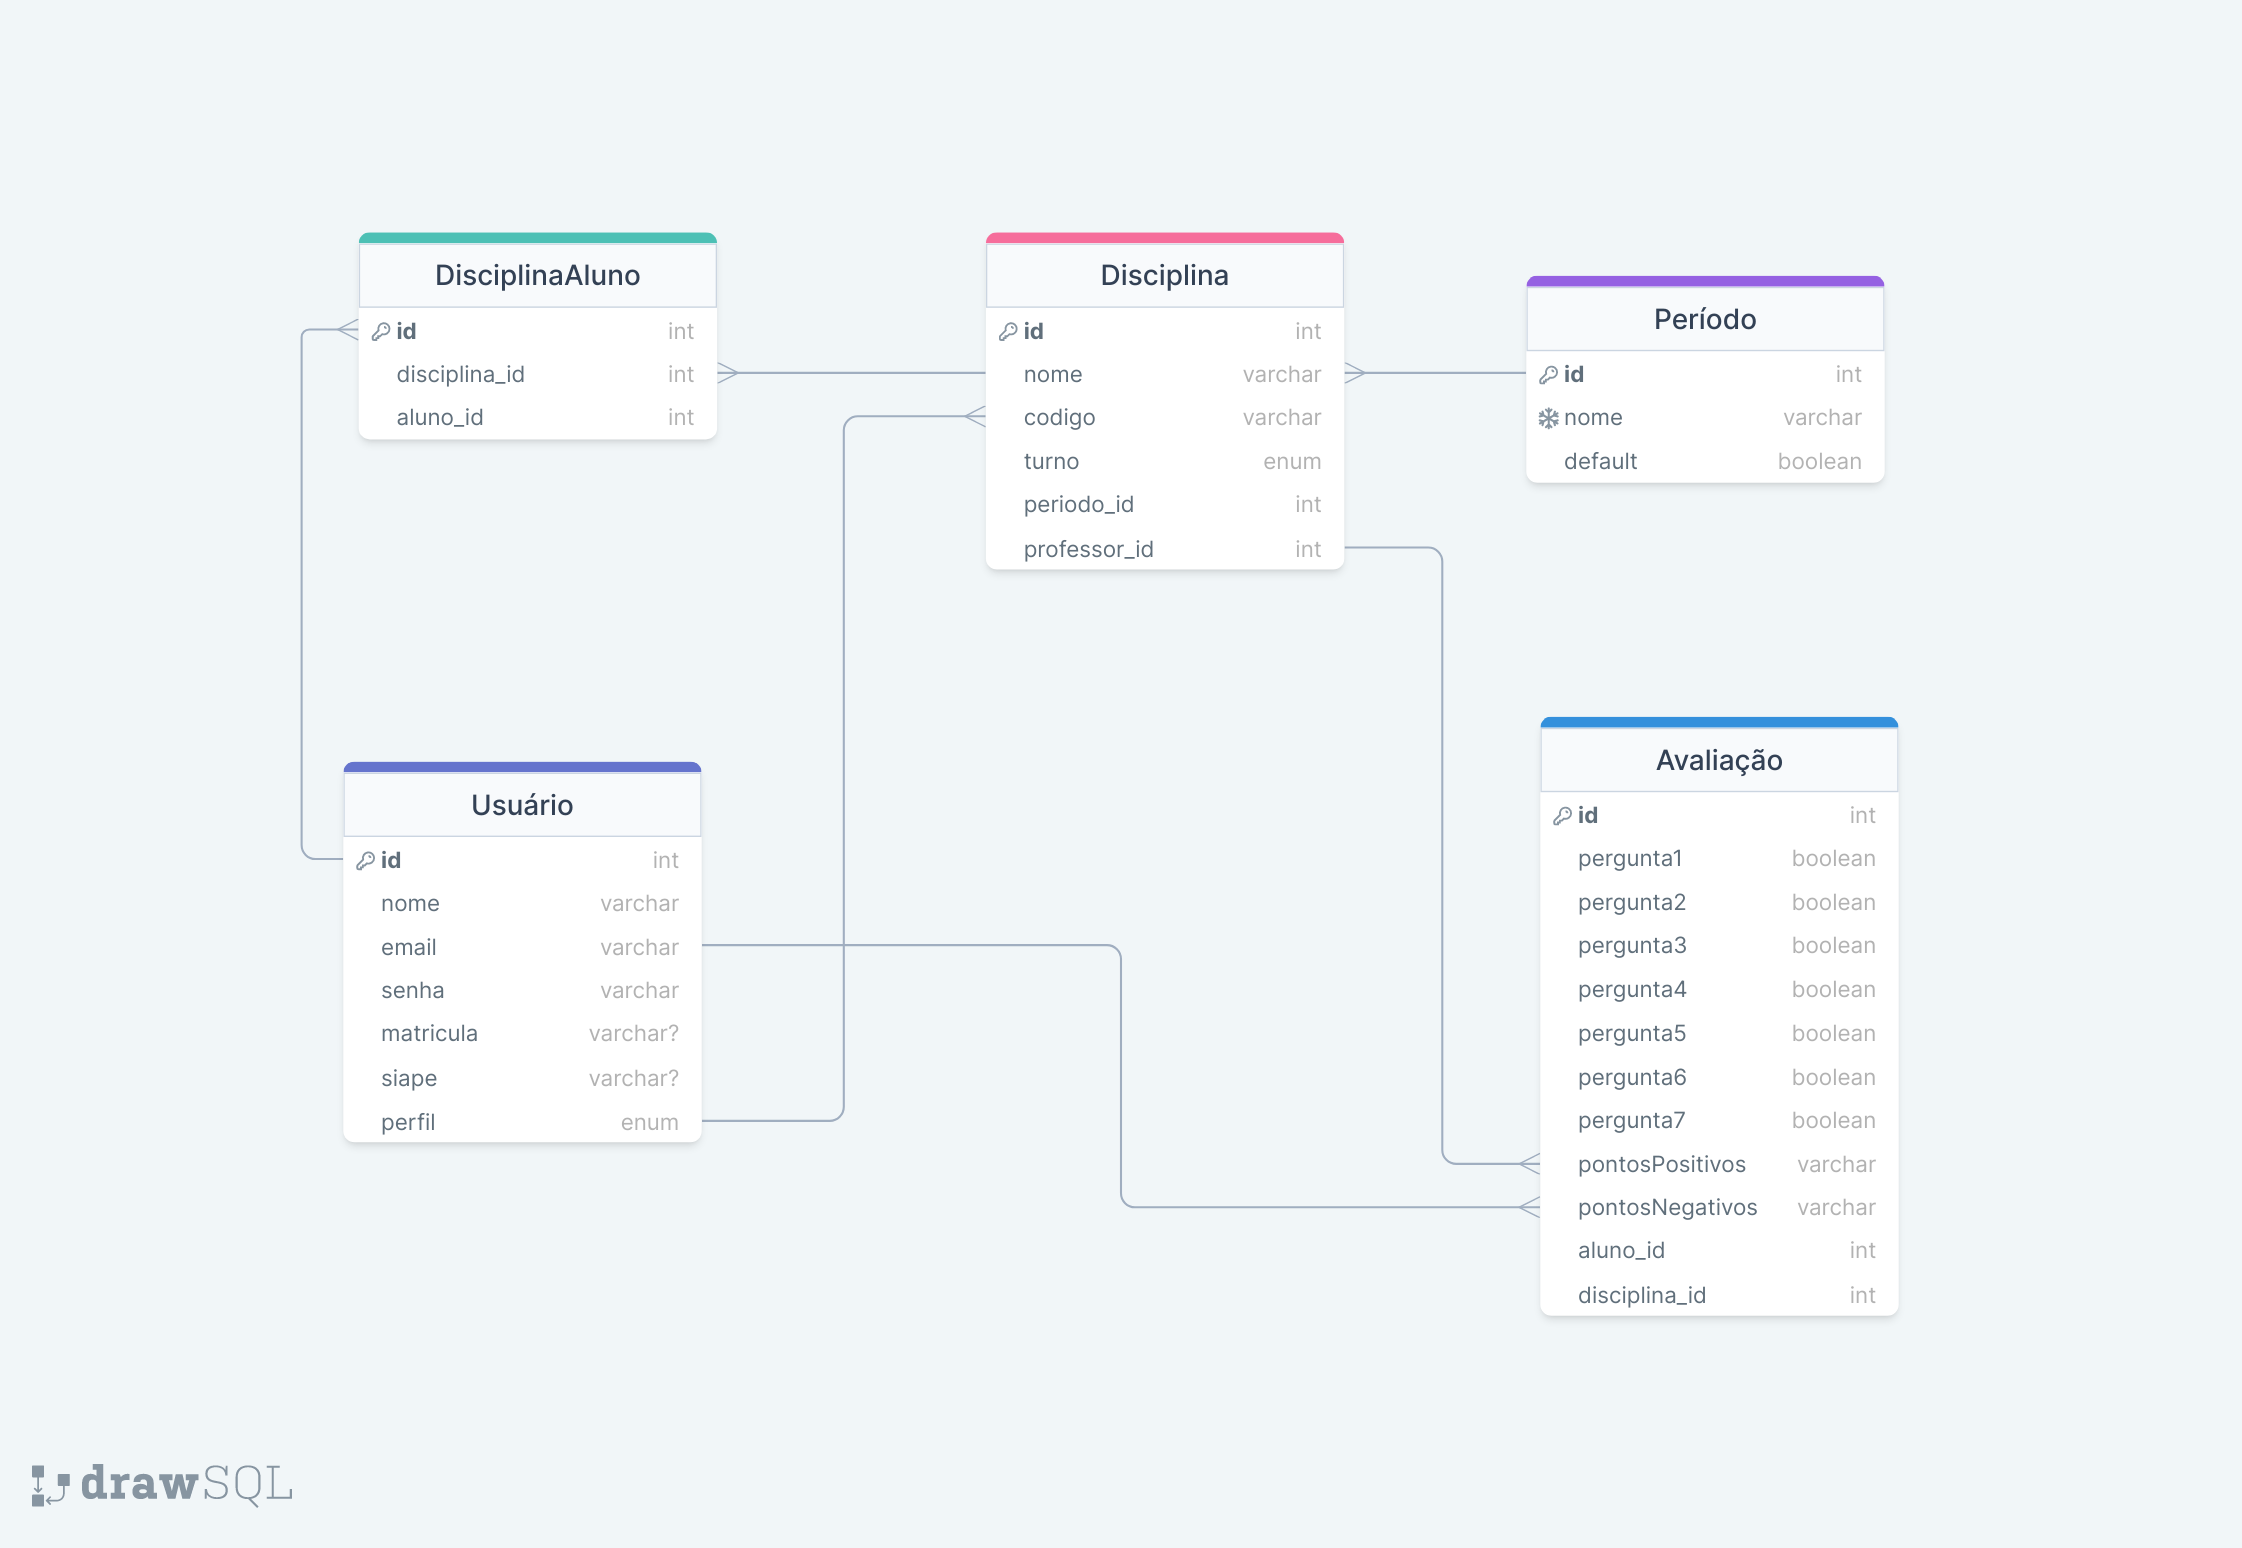
\includegraphics[width=1\textwidth]{imagens/diagrama-er.png}
  \caption{Diagrama ER}
  \label{fig:fig_diagrama_classe}
  \legend{Fonte: o autor.}
\end{figure}




%%%%%%%%%%%%%%%%%%%%%%%%%%%%%%%%%%%%%%%%%%%%%%%%%%%%%%%%%%%%%%%%%%%%%
% [1] - Cad. Cedes, Campinas vol. 29, n. 78, p. 257-269, maio/ago. 2009 257 Disponível em <http://www.cedes.unicamp.br>
% [2] - 
% - Importâncida da avaliação institucional no que diz respeito de detectar demandas/melhorias/pontos fracos
% - SINAES como medidor de qualidade de ensino superior
% - Avaliação interna abrange situações/necessidades mais específicas
% - 
%

% Esse capítulo será responsável por explicar como será a sua solução.
% Ele deverá explicar o problema em que a sua solução irá resolver.
% Nele irá conter COMO deverá ser a sua solução, ou seja, neste momento você não está preocupado com a implementação ou ferramentas.
% Aqui será relatado o problema e a sua proposta. 
% Nela será incluída a modelagem da solução, sua arquitetura e tudo o que for necessário para que o leitor consiga entender COMO será a solução e como ela resolverá o problema relatado.

% Além disso, uma parte fundamental, é tratar de trabalhos relacionados. Dependendo da forma de escrita, o trabalho relacionado pode estar explicado no capítulo de Fundamentação ou ser uma seção dentro da proposta antes de entrar na proposta em si.